\documentclass[]{article}

\begin{document}
\section{Bijlage Gebruikersdocumentatie}
Deze sectie zal een nieuwe gebruiker wegwijs maken in de visuele programmeer omgeving. Deze documentatie is onderverdeeld in enkele delen: programma creatie, menu en functionalieit hierin, debugging en de data editor.
\subsection{Installatievereisten}
AxeSki vereist Java versie 8 of hoger.
\subsection{Algemene uitleg programmeer taal}
\textbf{AxeSki} is een visuele programmeer omgeving. Het hoofddoel van de IDE is om event-based programma's te kunnen schrijven. Een gebruiker kan standaard programma's maken net zoals in andere programmeertalen. Een bijkomend voordeel is dat de gebruiker goed leert hoe event-based programming werkt.\\\\
De gebruiker werkt voornamelijk met \textbf{Events}, dit zijn informatiepakketten die in een programma rondgezonden kunnen worden tussen verschillende entiteiten. Deze events worden aangeduid door een unieke naam. De informatie die erin zit wordt ook aangeduid door een unieke naam binnen het event. \\\\
Vervolgens kan de gebruiker met behulp van programmeerstructuren een \textbf{klasse} opbouwen. Een klasse is een entiteit binnen het programma die kan reageren op bepaalde Events, en er ook zelf kan uitsturen. Deze programmeerstructuren omvatten de standaard programmeer constructies zoals een while-loop, if-condities, operaties, variabelen, etc. In een klasse bepaald de gebruiker hoe hij inkomende events afgehandeld. Een klasse kan ook terug events verzenden, hierin bepaald de gebruiker welke informatie in het te versturen event plaatst.

\subsection{Datatypes}
In de programmeer omgeving zijn drie verschillende datatypes beschikbaar. Namelijk Booleaanse waarde, Numerieke waarde en Strings. Ook kan er gebruik worden gemaakt van letterlijke waarden. 
\subsection{Programma creatie}
Een programma wordt opgebouwd in drie delen. Namelijk het aanmaken van Events, defini\"{e}ren van klasse en aanmaken van instanties en verbindingen maken tussen deze instanties. Alle drie de delen kunnen parallel worden opgebouwd. Elk deel gebeurt in een ander component van de GUI. Deze sectie helpt de gebruiker te werken met elk van deze componenten.
\subsubsection{Event creatie}
Zoals eerder vermeld kunnen instanties met elkaar communiceren via het doorsturen van Events. Naast de standaard beschikbare InputEvents zoals MousePressed kan de gebruiker zelf Events defineren. Deze Events zullen dan beschikbaar zijn voor de definitie van klassen.\\\\
In het Event creatie venster heeft de gebruiker aan de linkerkant een overzicht van alle Events die hij reeds gedefineerd heeft. Een nieuw Event toevoegen kan via de new Event knop. Het verwijderen kan via de ''Delete Event`` knop.\\\\
Bij het aanmaken van een nieuw Event zal een unieke naam moeten geven worden. Na het succesvol aanmaken van een Event kan het Event gedefineerd worden. Een Event kan gezien worden als een pakketje data dat verstuurd wordt. Om de data van een Event in te vullen of op te vragen moet de data verdeeld worden in verschillende variabelen. Deze variabelen worden Members genoemd.\\\\
De gebruiker kan Members toevoegen aan zijn Events door een unieke naam in te geven in het input veld onder de reeds bestaande members. Na het aanmaken kan het type van een member op elk tijdstip veranderd worden. Een Member kan verwijderd worden door op het rode kruisje te drukken.
\begin{figure}[H]
  \centering
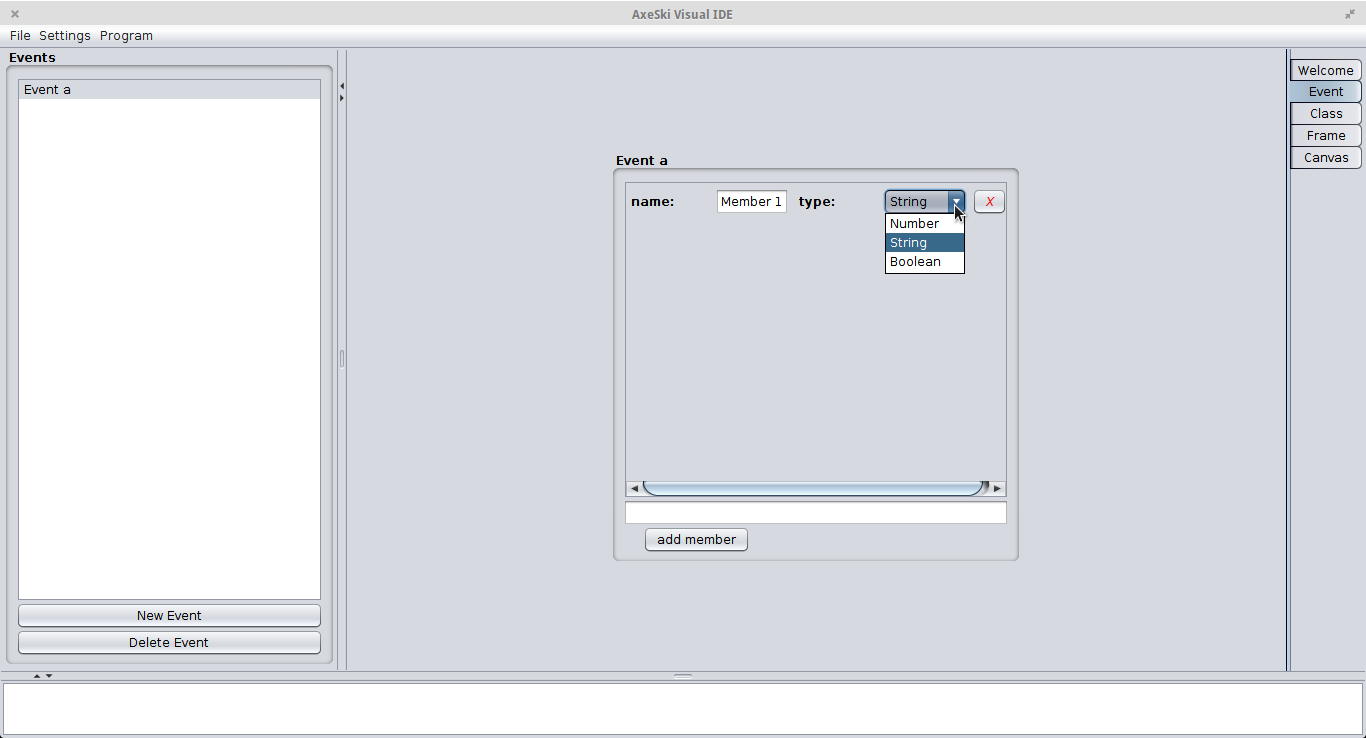
\includegraphics[scale=0.2]{Documentatie/images/EventView}
  \caption{EventView.} \label{EventView}
\end{figure}

\subsubsection{Klasse creatie}
In het klasse view kan er een nieuwe klasse worden toegevoegd door op de ''+`` tab te drukken. Hierna wordt gevraagd om een unieke naam te geven voor de nieuwe klasse. De naam van een klasse kan veranderd worden door rechts te klikken op de tab van de klasse waarvan men de naam wenst te veranderen. Het venster voor een klasse te cree\"{e}ren bestaan uit vier delen.
\begin{figure}[H]
  \centering
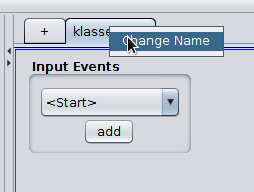
\includegraphics[scale=0.6]{Documentatie/images/changeclass}
  \caption{Veranderen klasse naam.} \label{KlasseView}
\end{figure}


\subsubsection{Blokken selectie}
Aan de linkerkant bevinden zich alle verschillende blokken die gebruikt kunnen worden. Deze blokken zijn onderverdeeld in verschillende categorieen. Deze staan kort vermeld in Sectie~\ref{blokkendoc}. Het selecteren van een blok kan door links op de gewenste blok te drukken. De huidige geselecteerde blok is zichtbaar in de linkerboven hoek van dit venster.\\\\ Als een blok geselecteerd is kan deze op het paneel worden geplaatst van een klasse. De selectie blijft actief tot de gebruiker een blok versleept of tot de gebruiker de selectie ongedaan maakt. Dit kan door rechts op het paneel te drukken de ''deselect block`` optie te kiezen. Rechts klikken op een blok zal de optie ''remove block`` tonen. Deze optie verwijderd de volledige groep blokken waarvan de aangeklikte blok deel van uitmaakte als ook de blokken die deze blok zelf bevat.
\begin{figure}[H]
  \centering
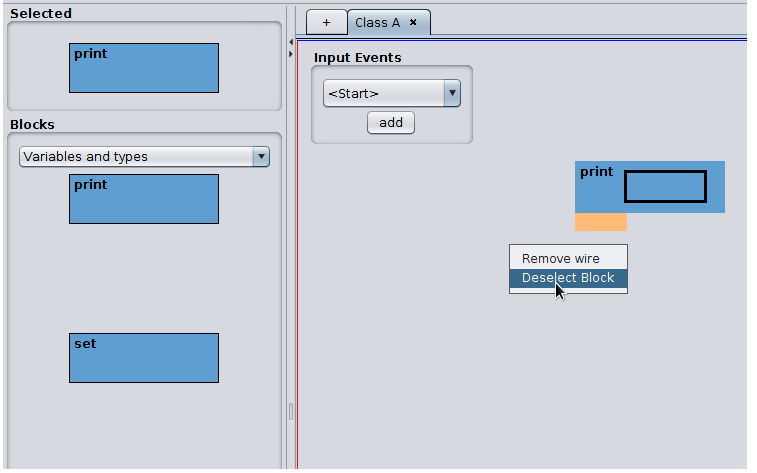
\includegraphics[scale=0.5]{Documentatie/images/select}
  \caption{Selected block.} 
\end{figure}

\subsubsection{Verslepen blokken}
Een blok kan versleept worden door deze vast te nemen met de muis cursor. Als de blok een body vormt zoals te zien in Figuur~\ref{bodydoc}, moet de bovenste blok vastgenomen worden. Als een andere blok in de body vastgenomen wordt, zal deze losklikken. Als een geneste blok vastgenomen wordt, zal deze ook losklikken uit zijn ouder blok. Dit is te zien in Figuur~\ref{bodydoc}. Hierbij toont de linkerkant een volledige body. Het midden toont hetgene losgeklikt wordt wanneer de print blok versleept zou worden. Het rechtergedeelte toont wat er gebeurt als de value blok versleept wordt.
\begin{figure}[H]
  \centering
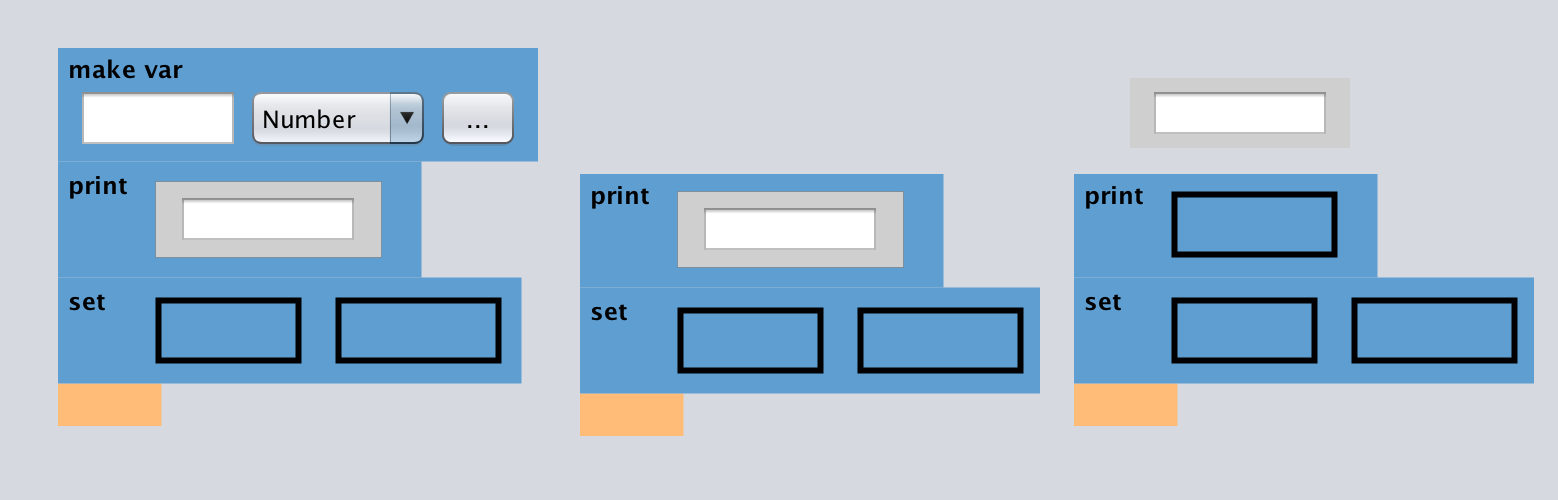
\includegraphics[scale=0.5]{Documentatie/images/losklikken}
  \caption{Losklikken blokken.} \label{bodydoc}
\end{figure}

Als een blok versleept wordt, zal deze doozichtig worden zoals te zien in Figuur~\ref{transparant}.
\begin{figure}[H]
  \centering
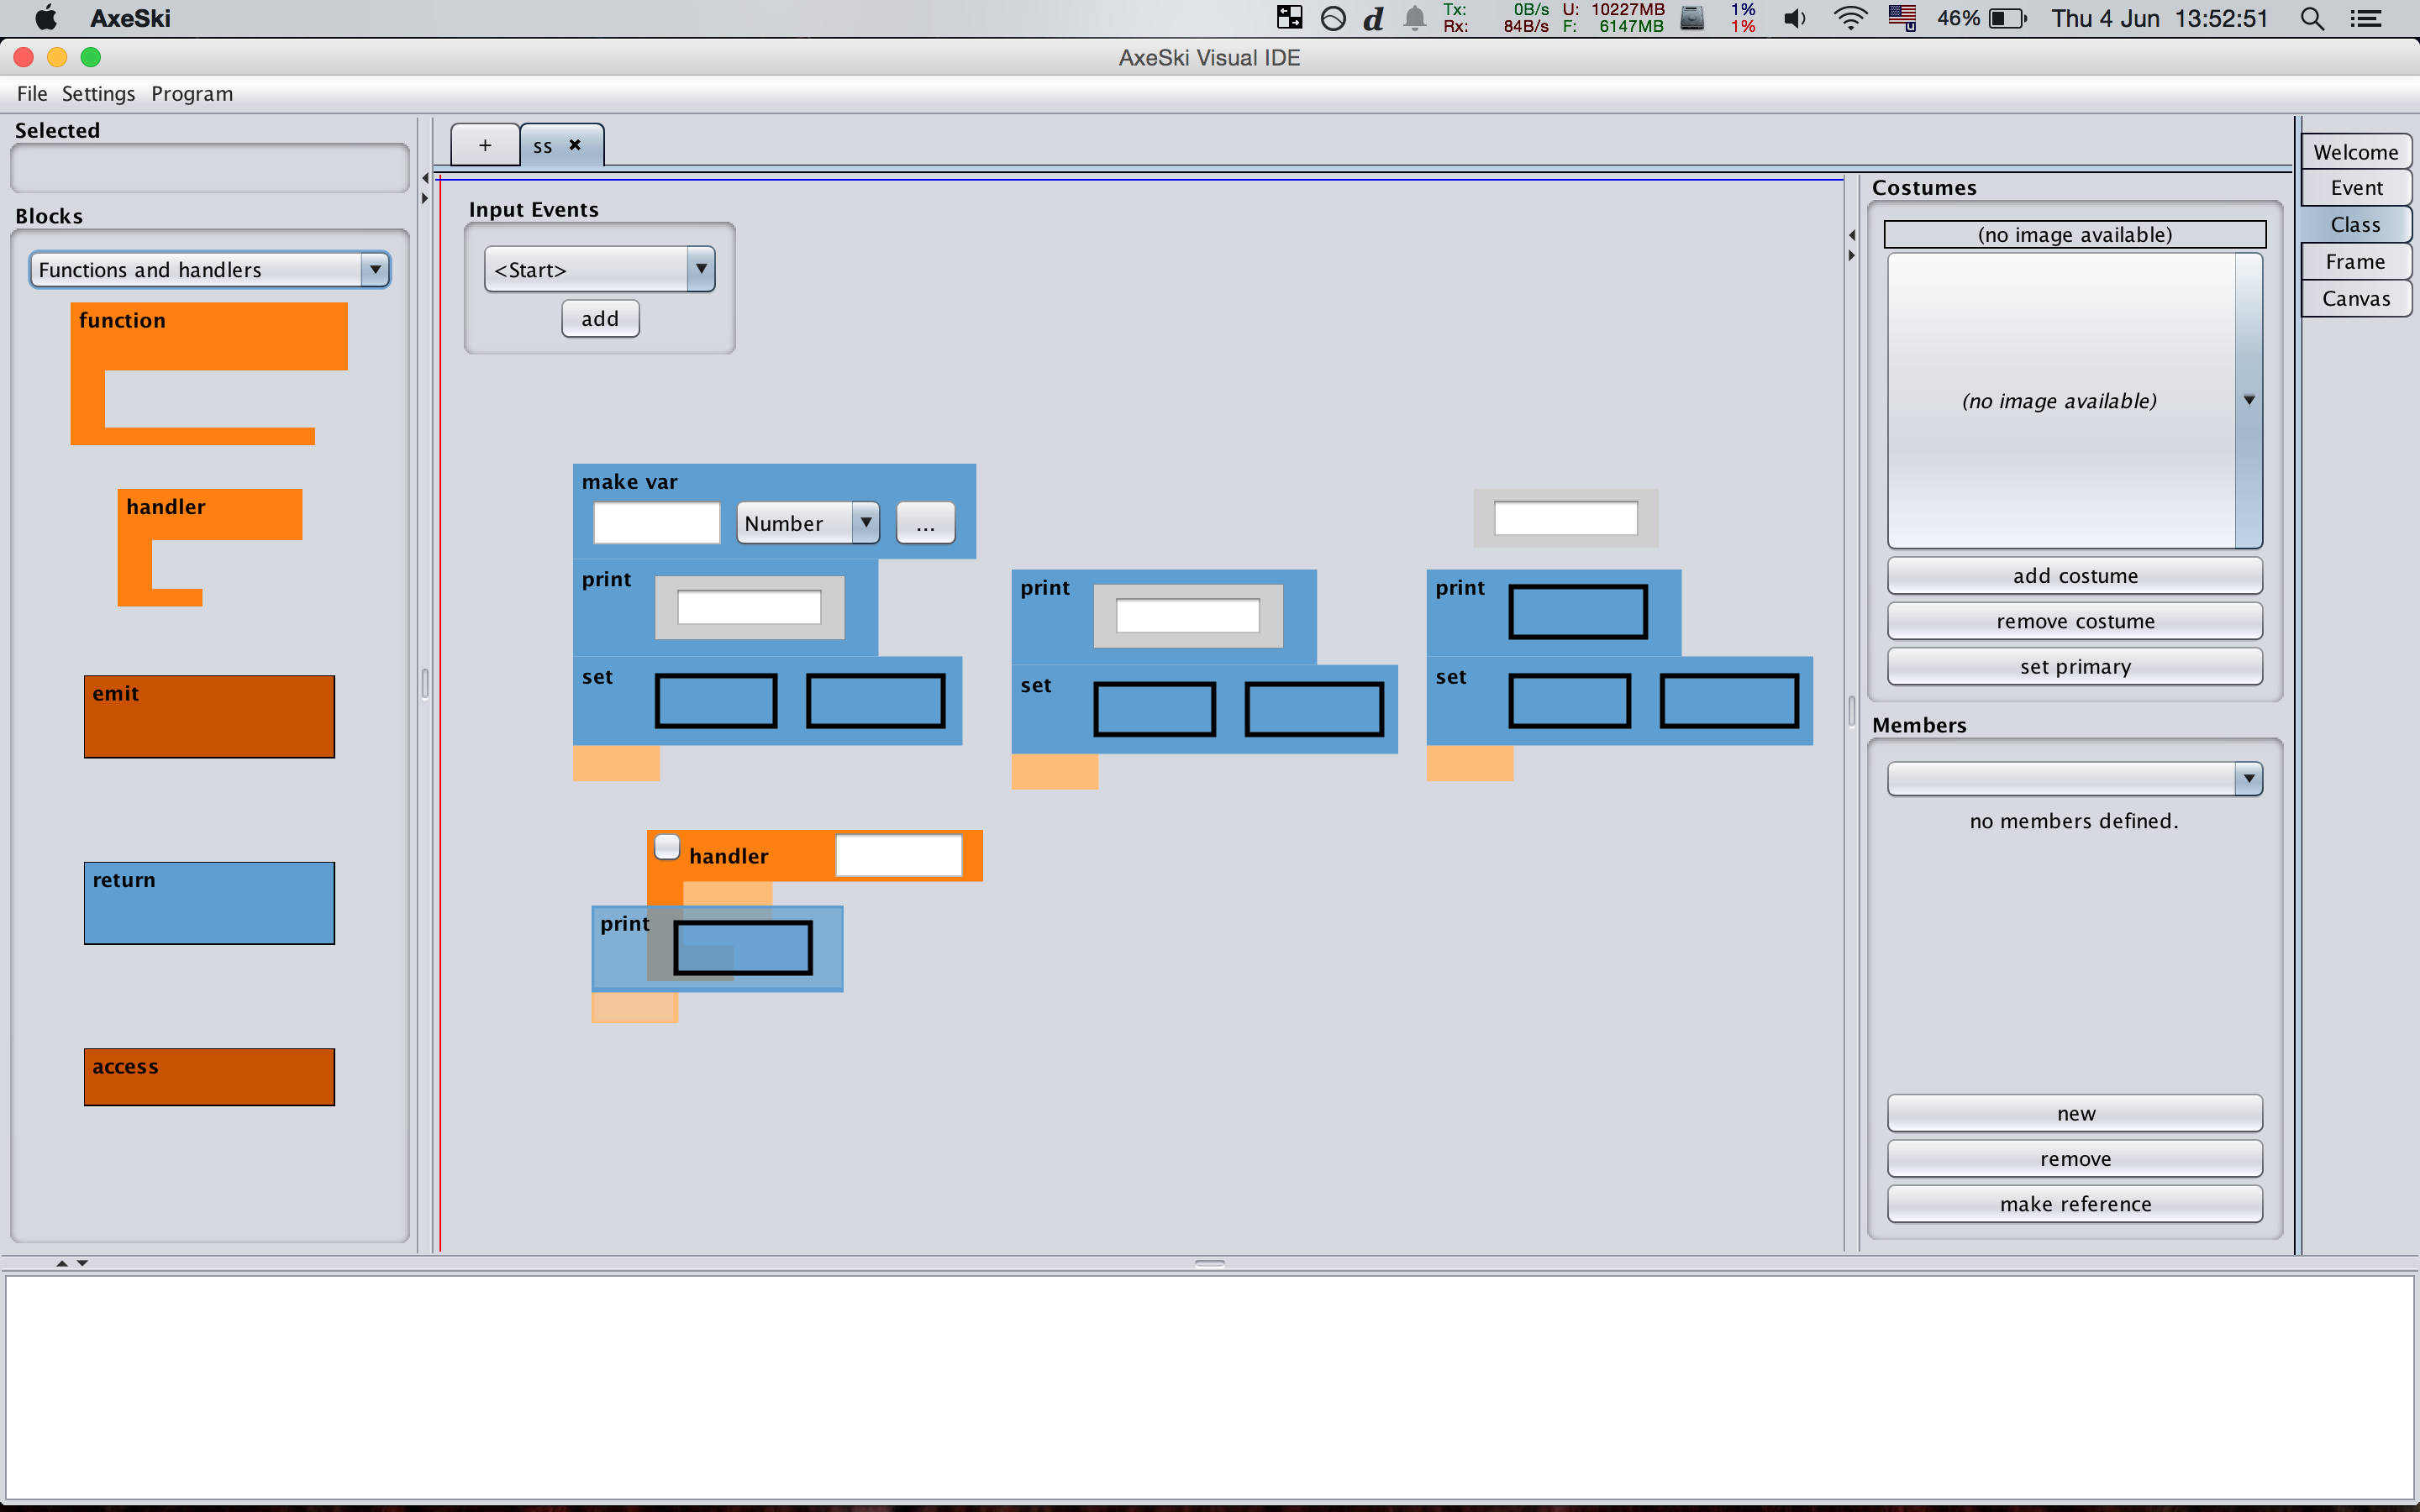
\includegraphics[scale=0.3]{Documentatie/images/transparent}
  \caption{Losklikken blokken.} \label{transparant}
\end{figure}

\subsubsection{Hulp menu}
De gebruiker kan een hulp menu openen voor een bepaalde blok. Deze actie kan uitgevoerd worden door de rechtermuisknop in te drukken en op de hulp optie te drukken zoals te zien in Figuur~\ref{hulpmenu}. Dit hulp menu geeft een korte samenvatting van de functie van die bepaalde blok, te zien in Figuur~\ref{hulp}
\begin{figure}[H]
  \centering
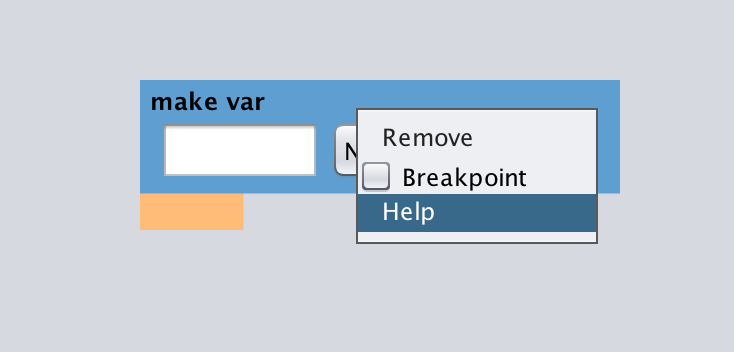
\includegraphics[scale=0.5]{Documentatie/images/hulpmenu.png}
  \caption{Hulp menu.} \label{hulpmenu}
\end{figure}\begin{figure}[H]
  \centering
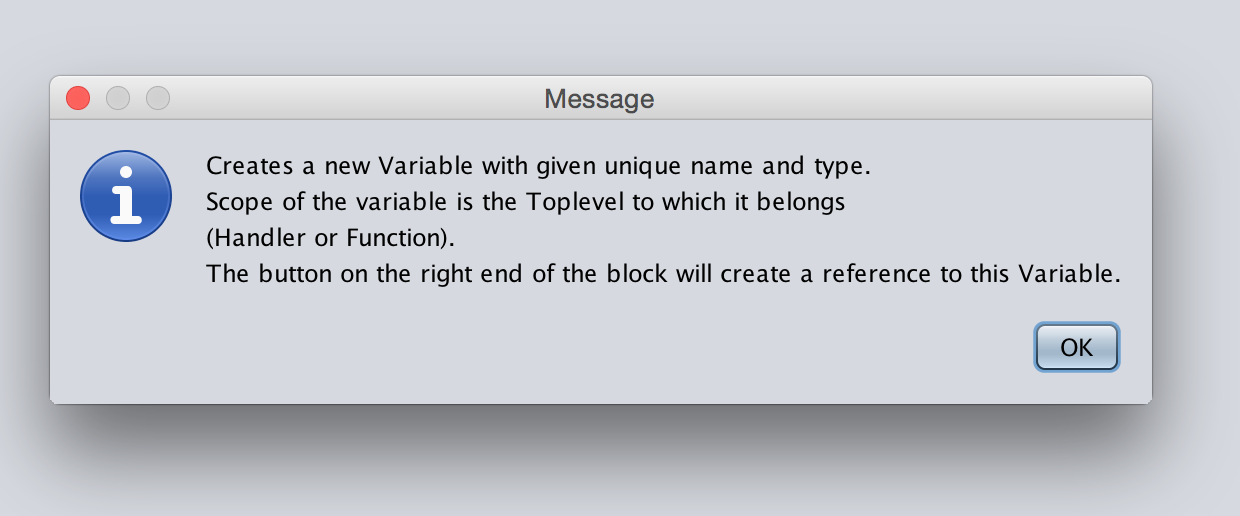
\includegraphics[scale=0.5]{Documentatie/images/hulp.png}
  \caption{Hulp dialog.} \label{hulp}
\end{figure}


\subsubsection{Klasse paneel} 
Het middelste deel van het scherm is gereserveerd voor het plaatsen van blokken. Hierin kan de gebruiker de werking van een klasse defini\"{e}ren. Dit paneel is van oneindige grootte. De gebruiker kan doorheen het paneel verplaatsen door het paneel vast te nemen en het weg te trekken.\\\\

\paragraph{Lokale variabele}
Binnen een functie of handler kan er gebruik worden gemaakt van variabelen. Deze kunnen aangemaakt worden doormiddel van een MakeVar-blok en deze toe te voegen aan een functie of handler. De variabele bestaat dan enkel in de scope van de functie of handler. De naam van die variabele moet dus ook uniek zijn in die scope. Als dit niet het geval is zal de de MakeVar-blok die de nieuwe variabele defini\"{e}rt een rode rand krijgen zoals te zien in Figuur~\ref{Variabele}.\\\\
Om gebruik te maken van een variabele kan er een referentie gemaakt worden naar de variabele. Dit gebeurt via de knop op het einde van de MakeVar-blok. Zoals al eerder vermeld bestaat een variabele enkel in de scope of definitie waarin zich zijn definitie (MakeVar-blok) bevindt. Als een referentie zich in een andere scope bevindt dan zijn definitie zal de referentie een rode rand tonen zoals in Figuur~\ref{Variabele}.

\begin{figure}[H]
  \centering
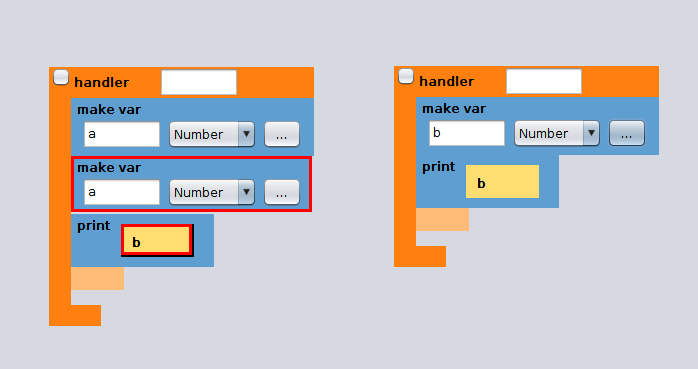
\includegraphics[scale=0.5]{Documentatie/images/errorvars}
  \caption{Variabele} 
  \label{Variabele}
\end{figure}

\paragraph{InputEvents en Handlers}
Standaard bevindt zich in de linkerboven hoek van het klasse paneel,het InputEvents paneel. Dit paneel geeft aan op welke inputEvents de klasse reageert. Bovenaan dit paneel bevindt zich een dropdown menu waarin alle standaard Events en door de gebruiker gedefineerde Events ter beschikking zijn. De gebruiker kan een inputEvent aan een klasse toevoegen door het gewenste Event te selecteren en op ''add`` te drukken. Het verwijderen van een inputEvent kan door op het kruisje naast de naam van het InputEvent te drukken.\\\\
Een Handler is een blok die de gebruiker kan gebruiken om een InputEvent op te vangen. Hij kan een Handler toekennen aan een InputEvent door op het vierkantje in de linkerboven hoek te drukken en daarna op het vierkantje naast de naam van het InputEvent te drukken.\\\\
Een verbinding kan verwijderd worden door het kabeltje aan te klikken en vervolgens op rechts te klikken op het paneel en de optie ''remove wire`` te selecteren. Voor een beter overzicht te hebben kan de gebruiker op de naam van het InputEvent drukken zodat de connectie aan de linker of rechter kant van het paneeltje staat.\\\\ 
Als een InputEvent members heeft kan deze opgevraagd worden doormiddel van een AccessBlock. Deze zal de members tonen van het InputEvent waarmee de Handler waarin hij zich bevindt mee verbonden is.\\\\
\begin{figure}[H]
  \centering
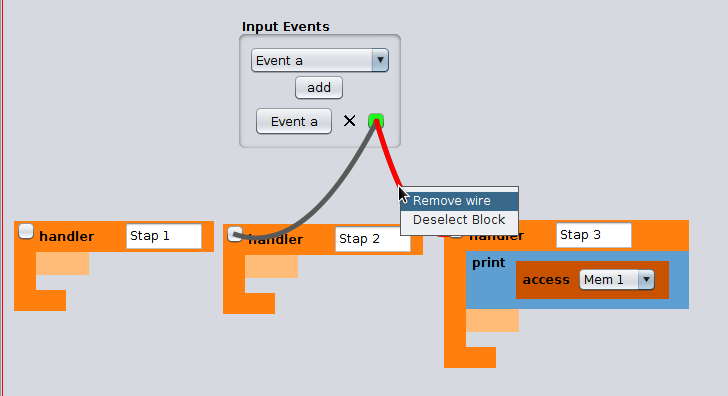
\includegraphics[scale=0.3]{Documentatie/images/handlerstap}
  \caption{Werking InputEvents en Handler.} 
\end{figure}

\paragraph{Functies}
Bij het selecteren van een Functie blok zal er een dialoog worden getoond waarin de gebruiker de functie header kan beschrijven. Hierin zal het het elke parameter van de functie moeten defini\"{e}ren. Alsook het returntype van de functie. Na het voltooien van deze dialoog kan de gebruiker de functie verder invullen.
\begin{figure}[H]
  \centering
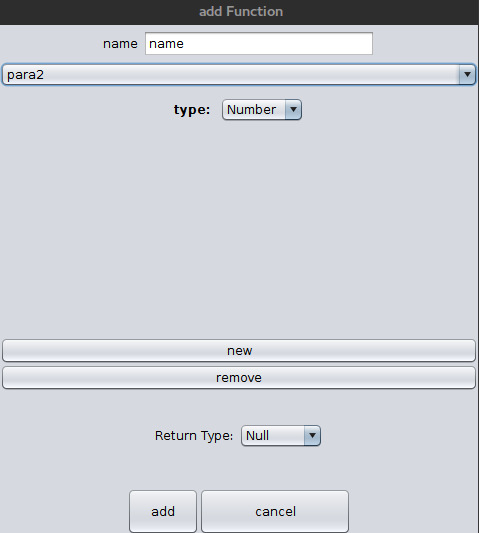
\includegraphics[scale=0.4]{Documentatie/images/functiondialog}
  \caption{Aanmaken van een functie.} 
\end{figure}

Het type van een parameter kan worden verkregen door te hoveren over de naam van de parameter. Een referentie naar een parameter kan worden gecree\"{e}rd door op de naam van de parameter te drukken.\\\\
Een functie oproep naar een functie kan worden aangemaakt door op het vierkantje te drukken dat zich na de laatste parameter van de functie blok bevindt.\\\\
\begin{figure}[H]
  \centering
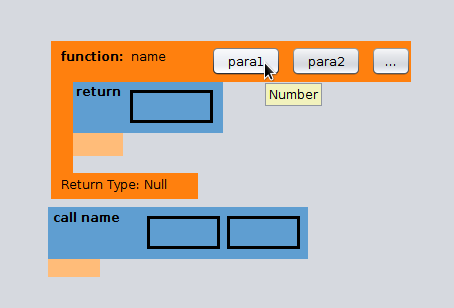
\includegraphics[scale=0.4]{Documentatie/images/functie}
  \caption{Functie blok en functie aanroep blok.} 
\end{figure}

\paragraph{Typechecking}
Bij het gebruik van blokken waarbij enkel bepaalde types toegelaten zijn, geeft het programma feedback over de types. 
Dit gebeurt doormiddel van een rode rand. Deze error verhinderen echter het uitvoeren van het programma niet. Bij de uitvoering zal in de console een gepaste error weergeven worden.\\\\
\begin{figure}[H]
  \centering
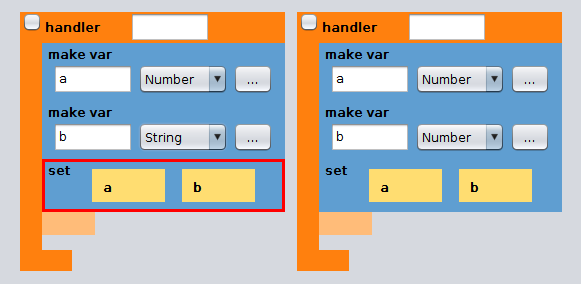
\includegraphics[scale=0.5]{Documentatie/images/typecheckError}
  \caption{Typechecking} 
\end{figure}
Voor een blok specifieke toegelaten blokken kan er naar de help functie van een blok worden gekeken. Voor de mogelijke combinaties van het gebruik van een binaire of unaire operatie kan de tabel in Figuur~\ref{operatortable} geraadpleegd worden.
\begin{figure}[H]
  \centering
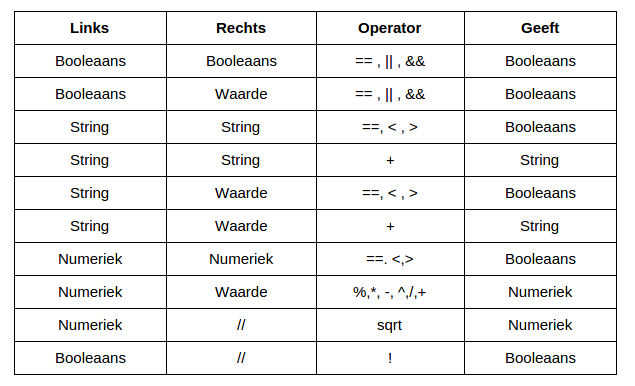
\includegraphics[scale=0.5]{Documentatie/images/operator}
  \caption{Operator combinaties.} 
  \label{operatortable}
\end{figure}

\paragraph{Kostuums}
In de rechterboven hoek van het klasse creatie venster bevindt zich een paneel waarin er kostuums aan een klasse kunnen worden toegevoegd. Het dropdown menu geeft een overzicht van alle reeds ingeladen kostuums. Deze kostuums kunnen dan in de klasse definitie gebruikt worden. Zo kan de gebruiker het uitzicht van een instantie van een klasse doen veranderen doormiddel van een set costume blok. Hierin kan een variabele of letterlijke waarde worden geplaatst. De waarde daarvan wordt dan bekeken als String. Als er een kostuum bestaat met die gegeven String als naam zal het gezet worden als uiterlijk voor die instantie.\\\\
Voor het selecteren van een standaard afbeelding van instanties van een klasse kan gebruik worden gemaakt van de ''set primary knop`` in het kostuum paneel. Het primaire kostuum wordt verkleint weergegeven bovenaan het paneel.\\\\
Bij het toevoegen van een nieuw kostuum zal een unieke naam moeten worden gekozen. Bij het mislukken van inladen of selecteren van een niet ondersteund bestandstype zal er geen afbeelding worden getoond. Het verwijderen van een kostuum kan door de ''remove`` knop te gebruiken. Dit zal het huidige geselecteerde kostuum in het dropdown menu verwijderen. Als dit kostuum het primaire kostuum was, zal het eerste kostuum als primair worden geplaatst.
\begin{figure}[H]
  \centering
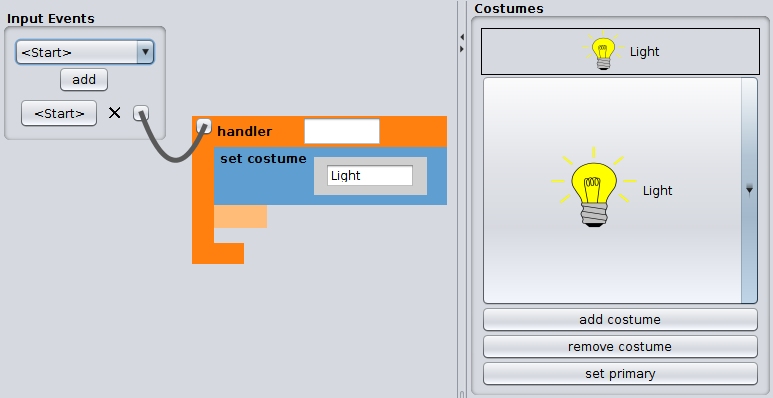
\includegraphics[scale=0.4]{Documentatie/images/costume}
  \caption{Kostuum paneel.} 
\end{figure}
\paragraph{Member variabelen}
Onder het Costume View bevindt zich het paneel voor member variabelen. Deze variabelen zijn beschikbaar dooreen de hele klasse. Om een referentie naar een member variable aan te maken, kan de gebruik de gewenste member selecteren en op ''make reference`` drukken. De geselecteerd blok (linksboven) toont nu een variable blok. Deze kan de gebruiker plaatsen op het panel zoals andere blokken. Een member variable zijn type kan aangepast worden via het dropdown menu.

\subsubsection{Console}
Er is een console aanwezig waar de gebruiker output naar kan schrijven.  Error output zoals variabelen die niet gevonden worden, worden in rode tekst uitgeprint. Standaard output wordt geprefixed door \texttt{[IDE]}. 
\begin{figure}[H]
  \centering
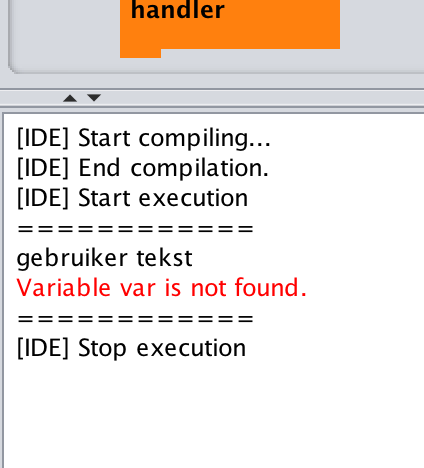
\includegraphics[scale=0.65]{Documentatie/images/console}
  \caption{Console output.} 
\end{figure}


\subsubsection{Instanties en verbindingen}
Deze sectie beschrijft hoe een gebruiker instanties van klassen kan aanmaken. En hoe hij de communicatie hier tussen kan defi\"{e}ren doormiddel van wires.
\paragraph{Aanmaken en verwijderen van een instantie}
Aan de linkerzijde bevind zich een lijst met alle bestaande klasse. Bij het aanklikken van een klasse zal deze geselecteerd worden. Hierna kan er op het paneel gedrukt worden om een instantie van de geselecteerde klasse aan te maken. Er zal gevraagd worden aan de gebruik om een unieke naam te geven voor een instantie. Een instantie kan verwijderd worden door rechts te klikken op een instantie en de optie ''remove`` te selecteren.
\begin{figure}[H]
  \centering
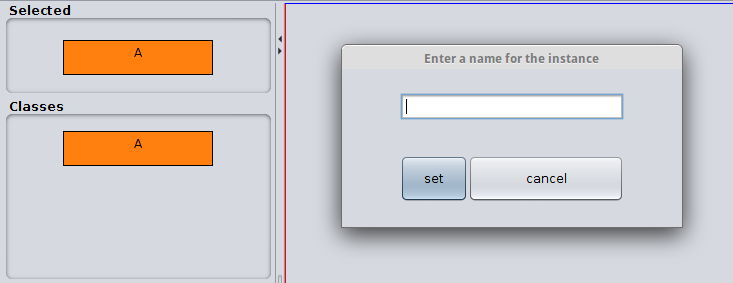
\includegraphics[scale=0.4]{Documentatie/images/makeinstance}
  \caption{Aanmaken van instantie.} \label{instanceCreation}
\end{figure}
\paragraph{Verbindingen tussen instanties}
Instanties kunnen Events naar elkaar sturen via wires. Wires kunnen enkel verbonden worden tussen dezelde Input- en OutputEvents van hetzelfde type. De gebruiker kan dit door het vierkantje naast een eventnaam van een InputEvent aan te klikken en vervolgens hetzelfde te doen voor een OutputEvent van hetzelfde type.\\\\
Verbindingen kunnen verwijderd worden door een wire aan te klikken en vervolgens bij het rechtskikken de optie ''remove wire`` te kiezen.
\begin{figure}[H]
  \centering
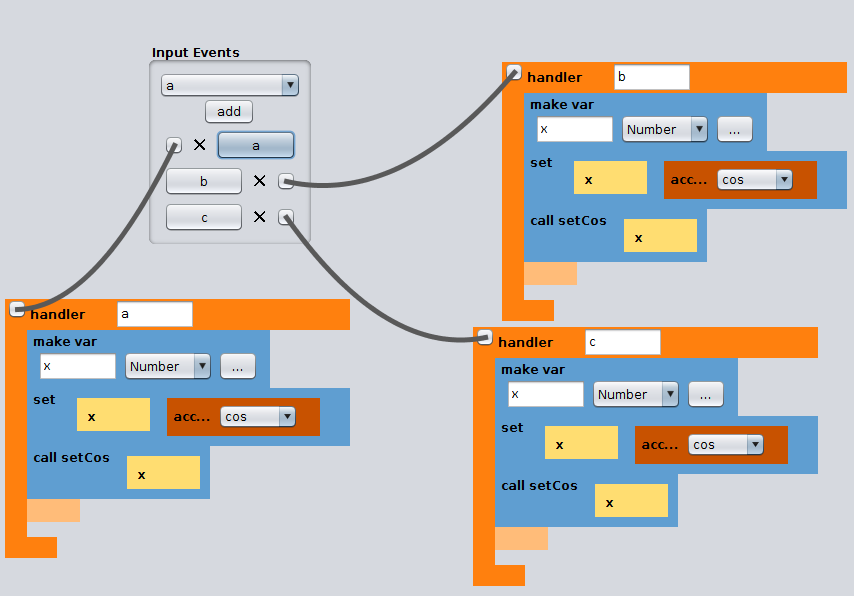
\includegraphics[scale=0.5]{Documentatie/images/wires}
  \caption{Events tussen instanties.} \label{wiresdoc}
\end{figure}
\paragraph{Filter}
Aan de linkerzijde van het Frame bevindt er zich een filter die alle bestaande Events in het programma bevat. Standaard is een Event aangevinkt. Dit betekend dat wires die dit type Event versturen getoond worden op het paneel. Als een Event is uitgevinkt zullen deze wires niet getekend worden.
\begin{figure}[H]
  \centering
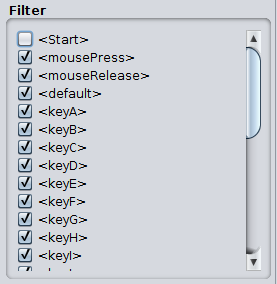
\includegraphics[scale=0.4]{Documentatie/images/filter}
  \caption{Filter.} \label{filterdoc}
\end{figure}

\subsection{Menu}
De user kan verschillende acties voltooien via het menu. Het filemenu is het menu waarmee de gebruiker interactie kan hebben met het opslaan en inladen van programma's. Zoals te zien in Figuur~\ref{runmenu} kan de gebruiker hier files openen en opslaan. Ook kan een nieuw project gestart worden. Dit zal alle huidige progressie verwijderen. Alle opties zijn beschikbaar via sneltoetsen.

\begin{figure}[H]
  \centering
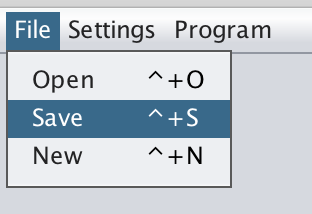
\includegraphics[scale=0.65]{Documentatie/images/menu/filemenu}
  \caption{File menu.} 
  \label{filemenu}
\end{figure}
In het settings menu kan de gebruiker de console leegmaken, ook kan hier de taal veranderd worden. Er is de keuze tussen Nederlands en Engels. Het wisselen tussen de talen is zoals te zien in Figuur~\ref{settingsmenu} ook beschikbaar via sneltoetsen.
\begin{figure}[H]
  \centering
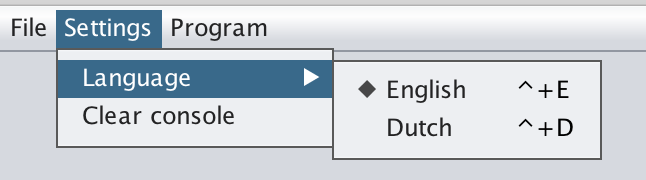
\includegraphics[scale=0.65]{Documentatie/images/menu/settingsmenu}
  \caption{Settings menu.} 
  \label{settingsmenu}
\end{figure}
De gebruiker kan het programma uitvoeren via dit menu. Er staan enkele opties geschikbaar. Een programma kan gecompileerd worden, kan uitgevoerd worden, kan gestopt worden en er kan doorheen het programma gestapt worden.
\begin{figure}[H]
  \centering
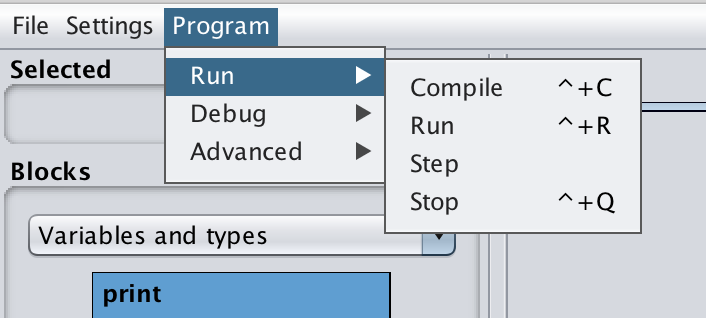
\includegraphics[scale=0.65]{Documentatie/images/menu/runmenu}
  \caption{Run menu.} 
  \label{runmenu}
\end{figure}
Het debugmenu heeft dezelfde functionaliteit als het runmenu. De gebruiker gebruikt hiermee het programma in debug modus. De functionaliteit van deze modus is uitgelegd in Sectie~\ref{debuggingdoc}
\begin{figure}[H]
  \centering
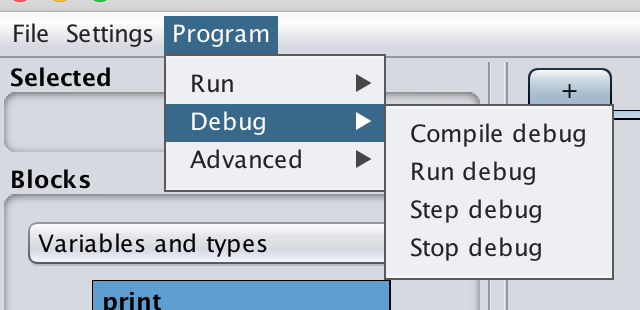
\includegraphics[scale=0.65]{Documentatie/images/menu/debugmenu}
  \caption{Debug menu.} 
  \label{debugmenu}
\end{figure}
Het data menu heeft een optie om de Data Editor aan te zetten of uit te zetten. 
\begin{figure}[H]
  \centering
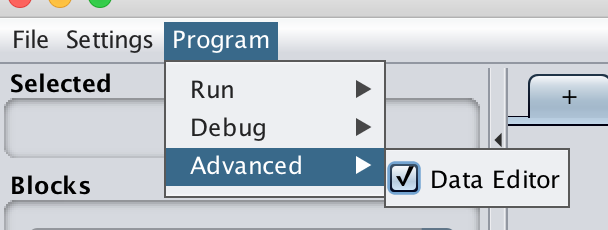
\includegraphics[scale=0.65]{Documentatie/images/menu/datamenu}
  \caption{Data menu.} 
  \label{datamenu}
\end{figure}

\subsection{Debugging}
\label{debuggingdoc}
In de IDE kan de gerbuiker debuggen. Blokken kunnen breakpoints bevatten. Dit kan getoggled worden door een optie in een popup menu. Dit menu wordt geopend door de rechtermuisklik in te drukken op een blok. Die blok krijgt vervolgens een paarse rand zoals te zien in Figuur~\ref{breakdoc}.
\begin{figure}[H]
  \centering
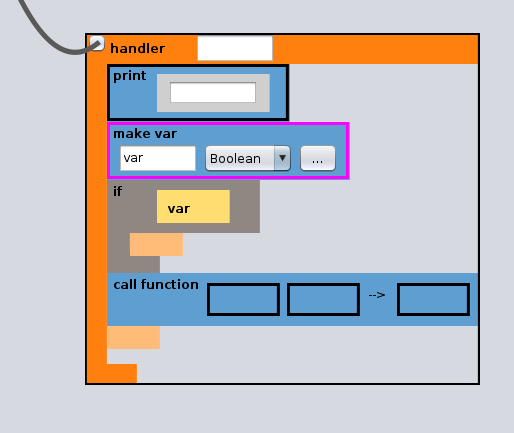
\includegraphics[scale=0.65]{Documentatie/images/break}
  \caption{Console output.} 
  \label{breakdoc}
\end{figure}

De gebruiker kan doorheen code stappen in debug modus. Dit toont een zwarte rand rond de momenteel uitvoerende blokken.
\begin{figure}[H]
  \centering
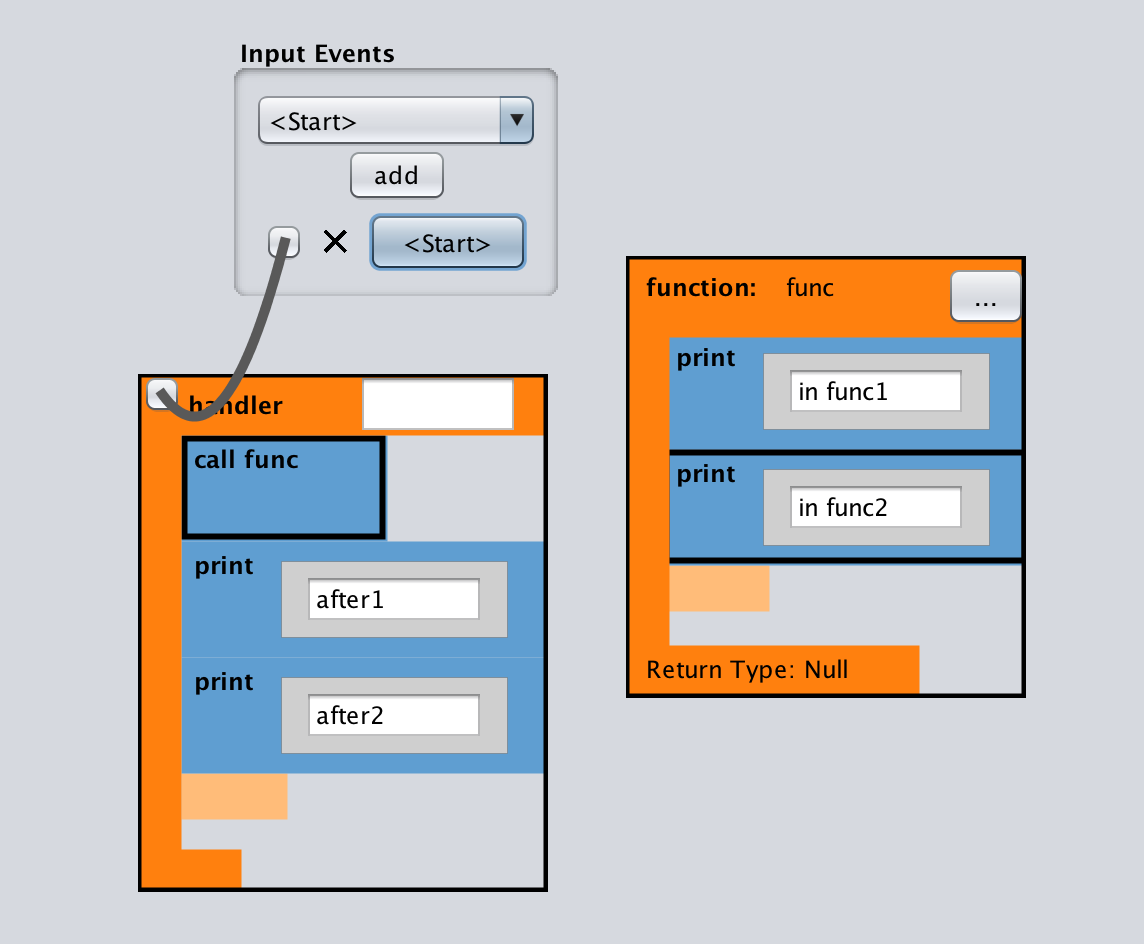
\includegraphics[scale=0.65]{Documentatie/images/debug}
  \caption{Console output.} 
  \label{debugdoc}
\end{figure}

\subsection{Data editor}
De Data Editor is een ingebouwde tekst editor om een programma te kunnen maken of aanpassen in zijn XML-vorm. Deze editor heeft syntax hightlighting zoals te zien in Figuur~\ref{dataeditordoc}. De data editor heeft zal aanpassingen doorvoeren naar de visuele views wanneer het view veranderd. Bij een foutieve XML zal een nieuw programma aangemaakt worden.
\begin{figure}[H]
  \centering
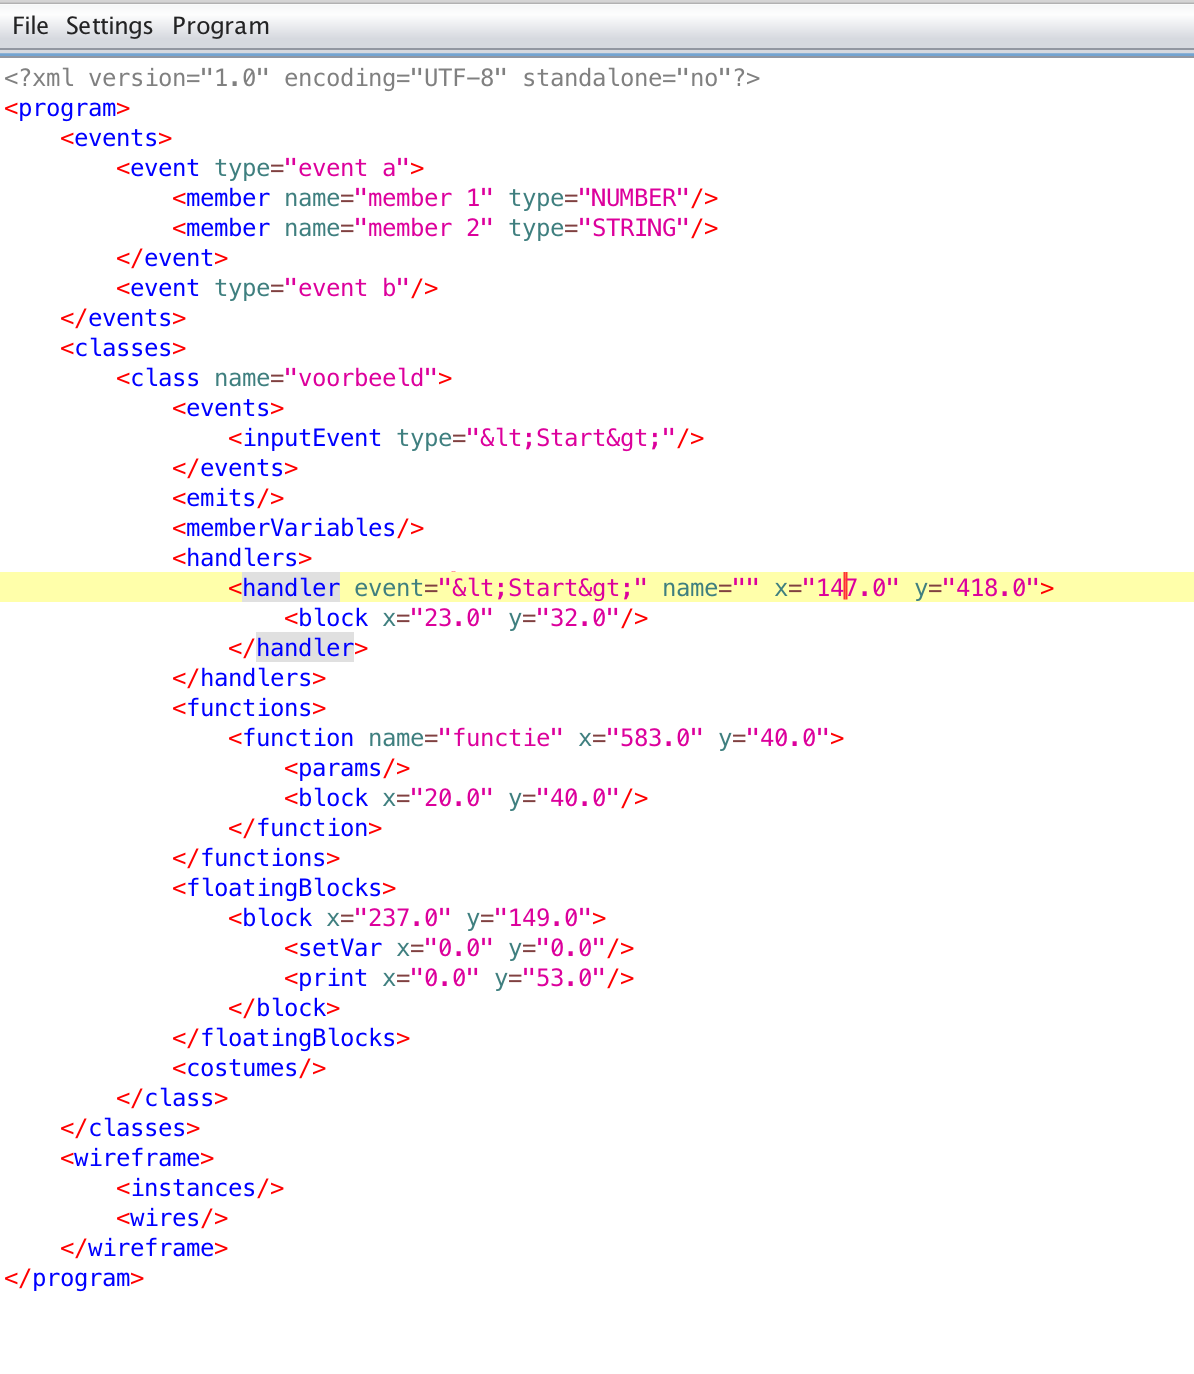
\includegraphics[scale=0.7]{Documentatie/images/dataeditor}
  \caption{Data Editor.} \label{dataeditordoc}
\end{figure}

\subsection{Overzicht van bestaande blokken}
\label{blokkendoc}
Deze sectie geeft een overzicht van alle blokken per categorie.
\subsubsection{Variabelen}
Bevat alle operaties om variabele aan te maken. Gelijk te stellen of uit te printen. 
\begin{itemize}
\item print
\item value
\item make var
\item set
\end{itemize}
\subsubsection{Condities}
Bevat alle conditie blokken.
\begin{itemize}
\item while
\item if
\item if-else
\item forever
\end{itemize}
\subsubsection{Functies en handlers}
Bevat handler en functie blokken. En operaties voor het opvangen van informatie uit een Event of het versturen van een Event.
\begin{itemize}
\item emit
\item access
\item function
\item handler
\item return
\end{itemize}
\subsubsection{Physics}
De blokken in deze categorie kunnnen gebruik worden voor de positie of uiterlijk van een instantie te veranderen.
\begin{itemize}
\item move
\item show
\item hide
\item set costume
\end{itemize}
\subsubsection{Locks}
Bevat blokken die gebruikt kunnen worden voor het locken en unlocken van variabelen.
\begin{itemize}
\item lock
\item unlock
\end{itemize}
\subsubsection{Trivia}
Bevat blokken die in geen connectie hebben met andere blokken.
\begin{itemize}
\item sleep
\end{itemize}
\subsubsection{Math}
Bevat blokken voor wiskundige bewerkingen alsook het aanmaken van een willekeurig getal.
\begin{itemize}
\item unaire operator
\item binaire operator
\item random
\end{itemize}
\subsubsection{String}
Bevat blokken voor operaties op variabele van het type String.
\begin{itemize}
\item length
\item concat
\item charAt
\end{itemize}


\end{document}